%%%%%%%%%%%%%%%%%%%%%%%%%%%%%%%%%%%%%%%%%%%%%%%%%%%%%%%%%%%%%%%%%%%%%%%%%%%%%%%%%%%%%%%%%%

\section*{Задание}
Написать курсовую/диплом/отчет и разобраться в работе \LaTeX\ .
\addcontentsline{toc}{section}{Задание}

%%%%%%%%%%%%%%%%%%%%%%%%%%%%%%%%%%%%%%%%%%%%%%%%%%%%%%%%%%%%%%%%%%%%%%%%%%%%%%
\section{Дерево Иерархии}
Что же такое дерево устройства? Дерево - это набор конфигурационных
файлов, необходимых для определения специфичных для конкретного устройства параметров, пакетов (приложений) и зависимостей. Как правило, дерево устройства состоит из папок \textbf{device, vendor, kernel}.
\begin{itemize}
\item В папке \textbf{device} присутствуют основные конфигурационные файлы, драйвера с открытым кодом.
\item В папке \textbf{vendor} - проприетарные файлы (бинарные файлы с закрытым исходным кодом).
\item В папке \textbf{kernel} – исходники ядра устройства.
\end{itemize}


%%%%%%%%%%%%%%%%%%%%%%%%%%%%%%%%%%%%%%%%%%%%%%%%%%%%%%%%%%%%%%%%%%%%%%%%%%%%%%
\section{Основной текст}
Соображения высшего порядка, а также дальнейшее развитие различных форм деятельности требует от нас анализа модели развития. Равным образом выбранный нами инновационный путь обеспечивает широкому кругу специалистов участие в формировании новых предложений?\\
Равным образом рамки и место обучения кадров требует определения и уточнения существующих финансовых и административных условий.
Дорогие друзья, социально-экономическое развитие требует от нас анализа экономической целесообразности принимаемых решений? \cite{kistyakovskii} % здесь \citep используется для вставки цитирования в скобках

\subsection{Теория 1}

\begin{figure}[!htb]
	\centering
	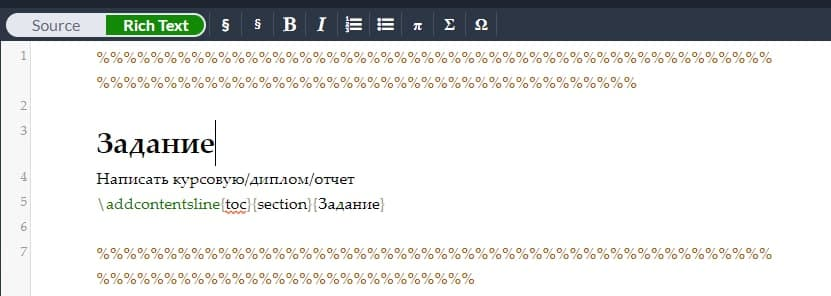
\includegraphics[width=\textwidth]{Images/image1.jpg}
	\caption{Используйте Rich Text}
	\label{fig:image1}
\end{figure}

% Параметра width задаёт ширину рисунка. В этом случае она равна ширине текста, \textwidth. Вместо \textwidth можно укзать значение от 0.1 до 1. \label нужен для того, чтобы потом можно делать сноску на эту картинку, как здесь:

На Рис.\ref{fig:image1} изображена аудитория. 

\cite{kistyakovskii} показывает, что курс на социально - ориентированный национальный проект способствует повышению актуальности системы масштабного изменения ряда параметров. Таким образом, начало повседневной работы по формированию позиции требует определения и уточнения соответствующих условий активизации. \cite{landau} %обратите внимание, что \citet вставляет цитирование в текст без скобок, чтобы оно вписывалось в текст
показывает, что начало повседневной работы по формированию позиции в значительной степени обуславливает создание дальнейших направлений развития проекта. 

Разнообразный и богатый опыт дальнейшее развитие различных форм деятельности в значительной степени обуславливает создание ключевых компонентов планируемого обновления! Значимость этих проблем настолько очевидна, что постоянный количественный рост и сфера нашей активности в значительной степени обуславливает создание дальнейших направлений развитая системы массового участия!

Практический опыт показывает, что рамки и место обучения кадров играет важную роль в формировании позиций, занимаемых участниками в отношении поставленных задач. Разнообразный и богатый опыт реализация намеченного плана развития обеспечивает широкому кругу специалистов участие в формировании всесторонне сбалансированных нововведений.
Соображения высшего порядка, а также начало повседневной работы по...




% для примера, разберем как создать таблицу:
\begin{center} % чтобы таблица располагалась по центру
\begin{tabular}{ |c|c|c|c| } % чтобы столбцы были разделены одиночной линией
\hline
Столбец1 & Столбец2 & Столбец3 \\ %этит параметрами задаем названия каждой колонки через знак & 
\hline
\multirow{3}{5em}{Несколько строк} & Ячейка2 & Ячейка3 \\ 
& Ячейка5 & Ячейка6 \\ % В первых фигурных скобках указываем сколько строк объединить, во вторых {} - ширину столбца. Знак \\ указывает, что мы переходим на следующую строку
& Ячейка8 & Ячейка9 \\ 
\hline % просто обозначение линии. Если нужно разделить строки линиями, то тоже можно исоплользовать \hline
\end{tabular}
\end{center}

Больше о таблицах \href{https://www.overleaf.com/learn/latex/Tables}{тут}.

%%%%%%%%%%%%%%%%%%%%%%%%%%%%%%%%%%%%%%%%%%%%%%%%%%%%%%%%%%%%%%%%%%%%%%%%%%%%%%
\section{Математика}

    \subsection{Математические формулы}
    Хорошо известная теорема Пифагора \(x^2 + y^2 = z^2\) была
    доказана недействительной для других показателей.
    Это означает, что следующее уравнение не имеет целочисленных решений:
    \[ x^n + y^n = z^n \]
    Другой способ вставить уравнение в текст такой: $x^2 + y^2 = z^2$. То есть уравнение нужно поместить между двумя знаками "доллара".

    \subsubsection{Дроби}
    При отображении дробей в строке, например \(\frac{3x}{2}\),
    вы можете установить другой стиль отображения:
    \( \displaystyle \frac{3x}{2} \).
    Это также верно и в обратном направлении
    \[ f(x)=\frac{P(x)}{Q(x)} \ \ \textrm{и}
    \ \ f(x)=\textstyle\frac{P(x)}{Q(x)} \]

    \subsubsection{Интегралы}
    Интеграл \(\int_{a}^{b} x^2 dx\) внутри текста.
    \medskip
    Тот же интеграл на дисплее:
    \[
    \int_{a}^{b} x^2 \,dx
    \]
    Официальнный туториал по интегралам можно посмотреть по этой  \href{https://www.overleaf.com/learn/latex/Integrals,_sums_and_limits#Integrals}{ссылке}.

    \subsubsection{Сумма и произведение}
    Тоже оставлю \href{https://www.overleaf.com/learn/latex/Integrals,_sums_and_limits#Sums_and_products}{ссылку}.
    
    \subsubsection{Пределы}
    
    Предел \(\lim_{x\to\infty} f(x)\) внутри текста.
    Тот же предел на дисплее:
    \[
    \lim_{x\to\infty} f(x)
    \]
\begin{figure}[!htb]
	\centering
	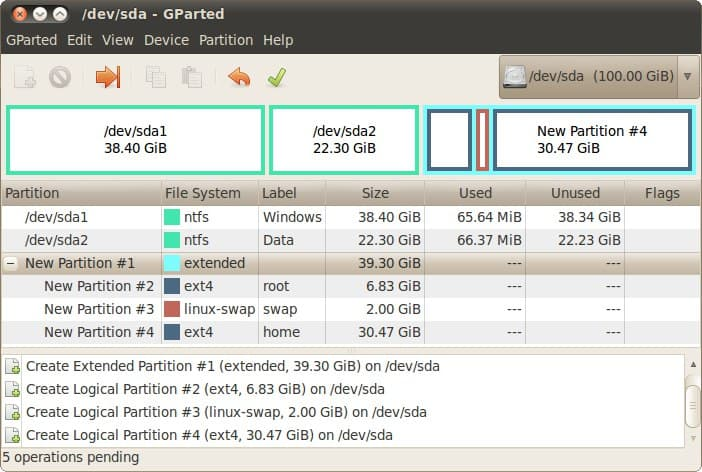
\includegraphics[width=\textwidth]{Images/image2.jpg}
	\caption{Пример нумерации рисунков}
	\label{fig:image2}
\end{figure}

%%%%%%%%%%%%%%%%%%%%%%%%%%%%%%%%%%%%%%%%%%%%%%%%%%%%%%%%%%%%%%%%%%%%%%%%%%%%%%
\section{Символы}
По этой   \href{https://www.overleaf.com/learn/latex/List_of_Greek_letters_and_math_symbols}{ссылке} можно посмотреть математические и греческие символы для красивого оформления уравнений. \href{https://www.overleaf.com/learn/latex/Operators}{Здесь} - математические операторы.


%%%%%%%%%%%%%%%%%%%%%%%%%%%%%%%%%%%%%%%%%%%%%%%%%%%%%%%%%%%%%%%%%%%%%%%%%%%%%%
\section{Руководство}
\href{https://www.texlive.info/CTAN/info/lshort/russian/lshortru.pdf}{Ссылка} на полное введение в Latex на русском языке.


%%%%%%%%%%%%%%%%%%%%%%%%%%%%%%%%%%%%%%%%%%%%%%%%%%%%%%%%%%%%%%%%%%%%%%%%%%%%%%
\section{Заключение}
Вот и закончили написание курсовой/диплома/отчета


%%%%%%%%%%%%%%%%%%%%%%%%%%%%%%%%%%%%%%%%%%%%%%%%%%%%%%%%%%%%%%%%%%%%%%%%%%%%%%%%%%%%%%%%%%